\section{Method - Drools in MPS}
\label{section:dsr_method}

Even though Drools is a relatively small DSL, we did not need to implement all the functionality to answer our questions.
For this reason, we first created a pilot study language to assess the possibilities of projectional solutions to our question.
We finally created a larger but incomplete version of Drools, in which we could create projections that would be recognisable to experienced Drools users.

\subsection{Really Simple Drools Language}
Our pilot study created a simple approximation of the Drools language to create our first projections. 
We called this language ``Really Simple Drools'' (RSD).
We describe this pilot study language here, as it contains many of the projections that we considered for our research question.

\subsubsection{Concepts}

\paragraph{\texttt{File}} RSD, like Drools itself, has a \texttt{File} Concept as its root node.
The \texttt{File} Concept only contains \linebreak\texttt{FactDeclaration} nodes and \texttt{Rule} nodes.

\paragraph{\texttt{FactDeclaration} and \texttt{FactProperty}} In Drools, a \texttt{FactDeclaration} Concept represents a Java Bean with its child properties, which can also have their child properties, ad infinitum.
In RSD, we limited properties to allow only boolean values.
We decided this because fact selection is a predicate and thus can only return a boolean.
By only allowing boolean values, we also simplify the operations allowed on a \texttt{FactProperty} node.

\paragraph{\texttt{Rule}} We only simulated the Left-hand side, or the ``when'' conditions, of a Drools Rule for the \texttt{Rule} Concept.
We believed this would provide us with compelling options for projections and did not want to overcomplicate this pilot project.

An RSD Rule consists of a collection of conditions.
Should all those conditions return ``true'', then the \texttt{Rule} node is selected.

\paragraph{\texttt{AbstractCondition}} A condition operates on one or more \texttt{FactSelectors} nodes.
There are four condition Concepts - \linebreak\texttt{ExistsCondition}, \texttt{NotCondition}, \texttt{AndCondition}, and \texttt{OrCondition}.
The \texttt{ExistsCondition} and \texttt{NotCondition} Concepts are unary conditions and evaluate one \texttt{FactSelector} node.
The \texttt{AndCondition} and \texttt{OrCondition} Concepts evaluate two \texttt{FactSelector} nodes.

\paragraph{\texttt{FactSelector}} A \texttt{FactSelector} Concept consists of a reference to a \texttt{FactDeclaration} node and a collection of \texttt{AbstractPredicate} nodes.
If the \texttt{FactDeclaration} node exists and all the predicates evaluate to \texttt{true}, then the \texttt{FactSelector} evaluates to \texttt{true}.

\paragraph{\texttt{AbstractPredicate}} The predicate is an operation on a \texttt{FactProperty} node, to which the Concept has a reference.
Because \texttt{FactProperty} nodes represent a boolean value, the only predicate operations are ``And'', ``Or'', ``Is'', and ``Not''.

We realised this design in MPS.
As the aim was to attempt different projections, we did not initially optimise for editing.
The Structure is as shown in figure \ref{fig:RSDStructure}.
We have here translated our Conceptual design of the RSD into MPS Concepts.
There is an almost one to one relationship with our concept hierarchy diagram.
The one difference is that the references in the concept hierarchy diagram, represented by the dashed red lines, are represented in our MPS Structure by SmartRef Concepts \texttt{FactDeclarationSmartRef} and \texttt{FactPropertySmartRef}.

\begin{figure}[h]
    \centering
    \fbox{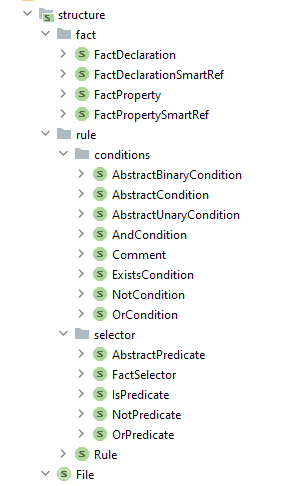
\includegraphics[width=0.40\textwidth]{Sections/images/RSRStructrure.png}}
    \caption{RSD Language Structure}
    \label{fig:RSDStructure}
\end{figure}

Figure \ref{fig:RSDDiagram} on page \pageref{fig:RSDDiagram} shows the Concept hierarchy for this straightforward implementation.

\begin{figure}[H]
    \centering
    \fbox{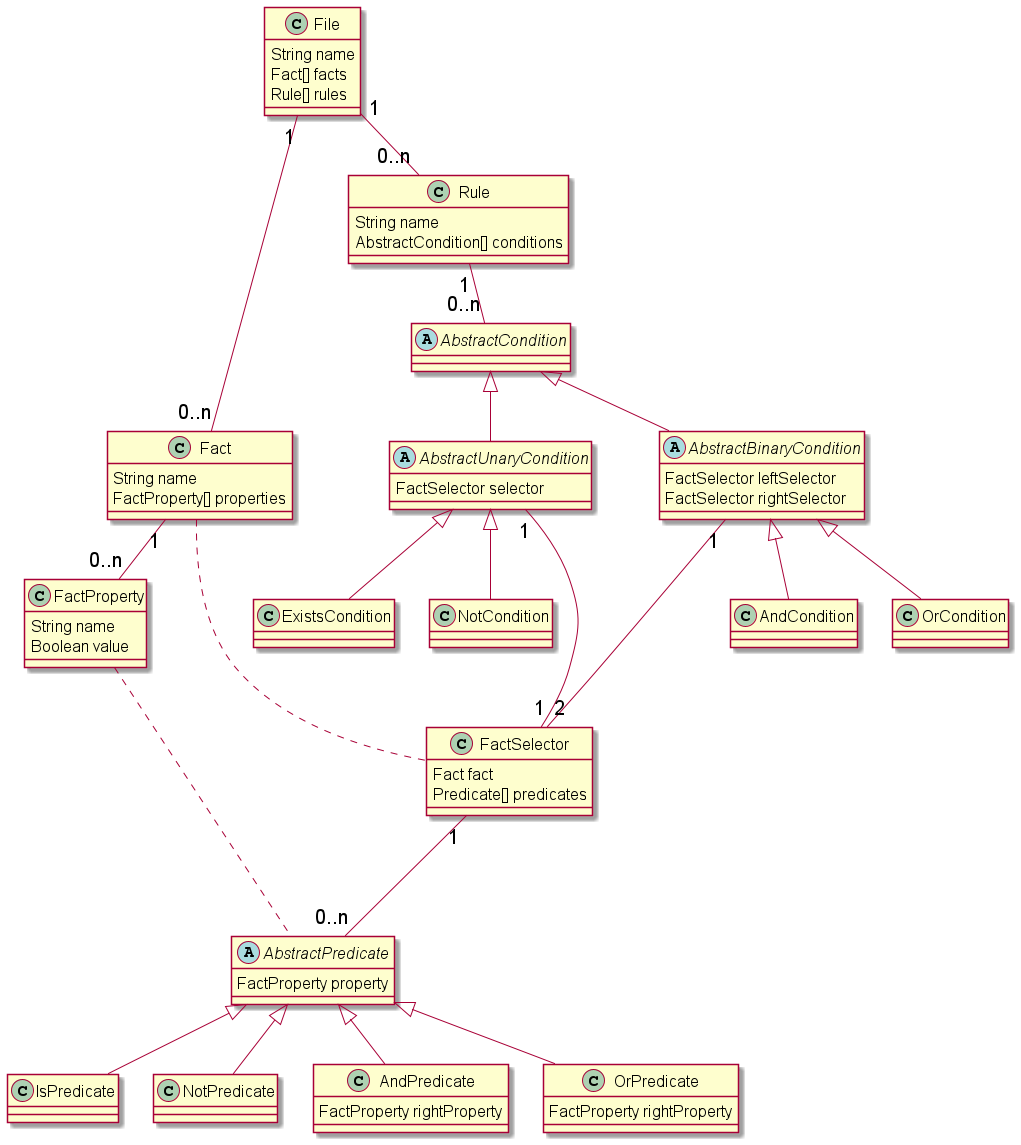
\includegraphics[width=0.95\textwidth]{Sections/images/ReallySimpleRuleLanguage4.png}}
    \caption{RSD concept hierarchy}
    \label{fig:RSDDiagram}
\end{figure}

We realised this design in MPS.
As the aim was to attempt different projections, we did not initially optimise for editing.
The Structure is as shown in figure \ref{fig:RSDStructure} on page \pageref{fig:RSDStructure}.
We have here translated our Conceptual design of the RSD into MPS Concepts.
There is an almost one to one relationship with our concept hierarchy diagram.
The one difference is that the references in the concept hierarchy diagram, represented by the dashed red lines, are represented in our MPS Structure by SmartRef Concepts \texttt{FactDeclarationSmartRef} and \texttt{FactPropertySmartRef}.


\subsubsection{Editors}

We show the definitions of the editors in figure \ref{fig:RSDEditors} on page \pageref{fig:RSDEditors}. 
The first editor describes the \texttt{File} Concept. 
It shows that the first line will have the text ``rule file name: '' followed by the file's name.
Following an empty line, there is a vertical listing of the \texttt{FactDeclaration} nodes stored in the ``facts'' child of the \texttt{File} node.
Thereafter is another empty line followed by a vertical listing of the \texttt{Rule} nodes stored in the ``rules'' child.

\begin{figure}[htbp]
    \centering
    \fbox{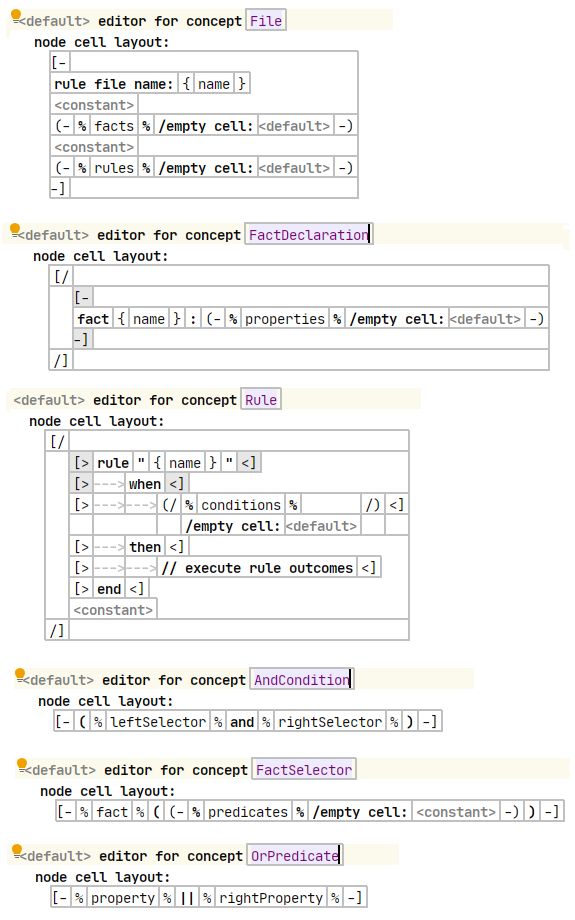
\includegraphics[width=0.66\textwidth]{Sections/images/RSREditors_P2.png}}
    \caption{Editors}
    \label{fig:RSDEditors}
\end{figure}

The next editor shown is the editor of the \texttt{FactDeclaration} Concept.
Each \texttt{FactDeclaration} node will be shown on a single line starting with the word ``fact'' followed by its name.
Then, between parentheses, a horizontal, comma-separated list of its child \texttt{FactProperty} nodes.

The subsequent editor describes the \texttt{Rule} Concept. 
The layout it describes is similar to that of a Drools rule, with the first line being ``rule'' followed by the \texttt{Rule} node name in inverted commas.
There is a hardcoded indented ``when'', followed by a further indented vertical list of the condition children, which are \linebreak\texttt{AbstractCondition} nodes.
At appropriate indentation levels, the conditions precede three hardcoded lines of ``then'', a place holder for the right-hand side of a standard Drools rule, and ``end''.

Next, we show one of the \texttt{AbstractCondition} Concepts, in this case, the \texttt{AndCondition} Concept.
This Concept editor displays the two \texttt{FactSelector} child nodes separated by ``and'' and surrounded by parentheses.

The editor for the \texttt{FactSelector} Concept displays the fact child, which is a \texttt{FactDeclarationSmartRef} node, for which we do not show its editor here, but in this case, shows the name of the \texttt{FactSelector} node that it is referencing.
The name precedes a horizontal, comma-separated list of the \texttt{AbstractPredicate} nodes stored in the predicate's children, encased in parentheses.

The final editor we show is an example of an \texttt{AbstractPredicate} Concept, specifically an \texttt{OrPredicate} Concept, which shows the two properties separated by a ``||'' symbol.
The properties are \texttt{FactPropertySmartRef} nodes, and they will just display the name of the \texttt{FactProperty} node to which they point.

\subsubsection{The Language}
We show the result of the editors in figure \ref{fig:RSDProgram}, which shows an example of our default Drools-like text projection. 
This projection is of the root AST of a \texttt{File} node called ``DossierSleutelbos''.
It has 4 \texttt{FactDeclaration} child nodes and 3 \texttt{Rule} child nodes.
The \texttt{FactDeclaration} nodes called ``Dossier'', ``Episode'', and ``Milestone'' each have two child \texttt{FactProperty} nodes, whilst ``DroolsContext'' has none.

The \texttt{Rule} node ``0'' has 2 \texttt{ExistsCondition} nodes containing \texttt{FactSelector} node children with \linebreak\texttt{FactDeclarationSmartRef} nodes referencing the \texttt{FactDeclaration} nodes ``Dossier'' and ``DroolsContext''.

The \texttt{Rule} node ``[WVGGZ/CM] start CM Procedure'' points to the ``Dossier'' \texttt{FactDeclaration} node, as well as having two predicates.
The first predicate is an \texttt{IsPredicate} node with a \texttt{FactPropertySmartRef} node pointing to the ``isWvGGZ'' \texttt{FactProperty} node.
The other predicate is a \texttt{NotPredicate} node pointing to the ``hasRunningEpisode'' \texttt{FactProperty} node.

The final \texttt{Rule} node has a complex nesting of \texttt{AbstractCondition} nodes.
The first is an \texttt{OrCondition} node containing an \texttt{ExistsCondition} node on its left-hand side and an \texttt{AndCondition} node on the right.
The right-hand side node contains an \texttt{ExistsCondition} node on both the left and right sides. 

\begin{figure}[h]
    \centering
    \fbox{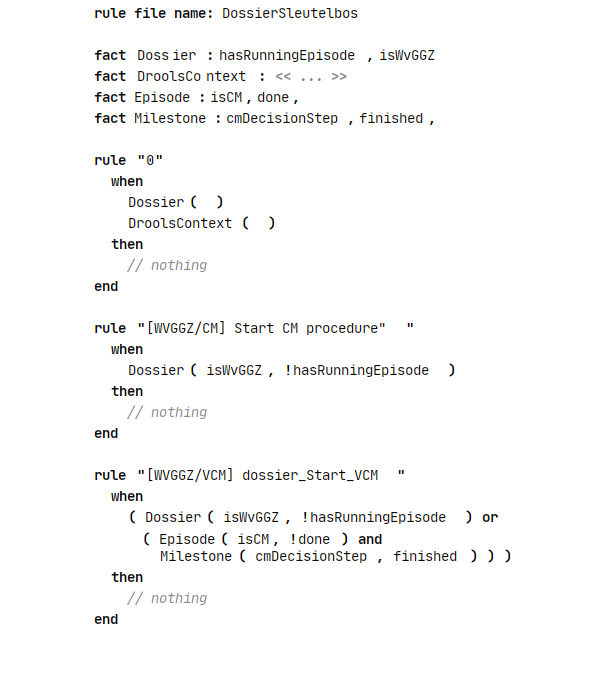
\includegraphics[width=0.66\textwidth]{Sections/images/RSRProgram_P.png}}
    \caption{RSD program}
    \label{fig:RSDProgram}
\end{figure}

\newpage
\subsubsection{Editing aids}
Part of our research question is using projections for reasoning about large files.
To answer this, we needed to simulate a large file.
To do this, we had to enter many \texttt{Rule} nodes.
As this becomes tedious, we added some editing aids, including substitute menus, to speed up the entry of Conditions, as shown in figure \ref{fig:RSDSubstituteMenu} on page \pageref{fig:RSDSubstituteMenu}.

\begin{figure}[h]
    \centering
    \fbox{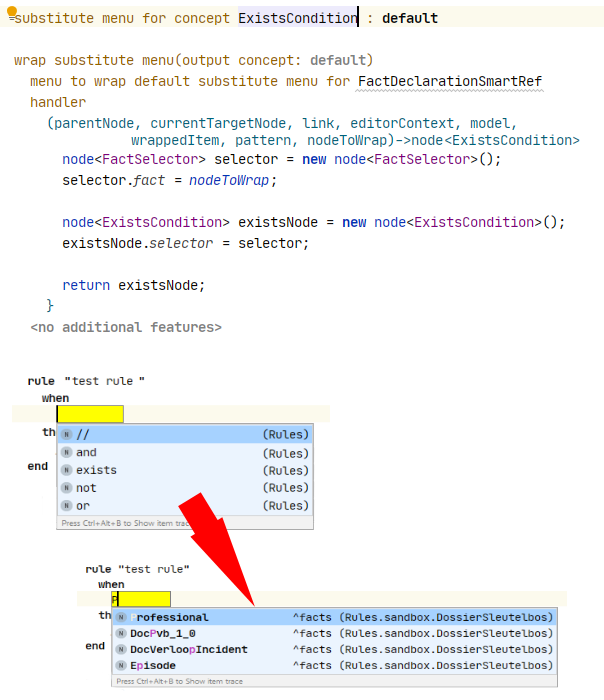
\includegraphics[width=0.66\textwidth]{Sections/images/RSRSubstituteMenu_P.png}}
    \caption{RSD substitute menu}
    \label{fig:RSDSubstituteMenu}
\end{figure}

This image shows that we originally had to select an \texttt{ExistsCondition} Concept and select the \linebreak\texttt{FactDeclaration} node for the Condition.
After adding the substitute menu, we could immediately select the \texttt{FactDeclaration} node we wanted, and it would automatically wrap it with an \texttt{ExistsCondition} node.

We show the code to do this in the section ``wrap substitute menu''.
What it does is when it encounters the possibility to input an \texttt{ExistsCondition} node in a menu, it replaces it with the default menu for the \linebreak\texttt{FactDeclarationSmartRef} Concept.
MPS handles SmartRefs in menus by showing all the possible reference items available.
When the user picks the reference item, this code will create a new \texttt{ExistsCondition} node with a new \texttt{FactSelector} node containing the chosen \texttt{FactDeclarationSmartRef} node to insert at that point in the AST.
This substitute menu saves several keystrokes, as otherwise, we manually first had to insert an \texttt{ExistsCondition} node followed by a \texttt{FactSelector} node before filling the \texttt{FactDeclaration} child.

Finally, we added a Constraint to scope the \texttt{FactProperty} references in \texttt{Predicate} Concept to the \linebreak\texttt{FactDeclaration} reference chosen in the \texttt{FactSelector} node.
This scope Constraint made it much easier to select \texttt{FactProperty} nodes in a \texttt{Predicate} node, as indicated in figure \ref{fig:RSDConstraint}, on page \pageref{fig:RSDConstraint}.

The figure shows that before adding the scoping constraint, it showed a list with dozens of potential \linebreak\texttt{FactProperty} nodes representing all the \texttt{FactProperty} nodes in the model.
After adding the constraint, it only shows the two \texttt{FactProperty} references associated with the \texttt{FactDeclaration} referenced in the \texttt{FactSelector}.
We achieve this scoping in the code in the scope method.
The code first finds the relevant \texttt{FactDeclaration} node from the \texttt{FactSelector} node we are at in the AST.
From this, it returns a list of properties as a \texttt{Scope}.

Thus, we have described the entire implementation of the Really Simple Drools Language.

After implementing the language, we wrote a program with many rules.
This program on which we will experiment with the different projections.

We discuss the alternative projections in the results section \ref{section:dsr_results}.

\begin{figure}[H]
    \centering
    \fbox{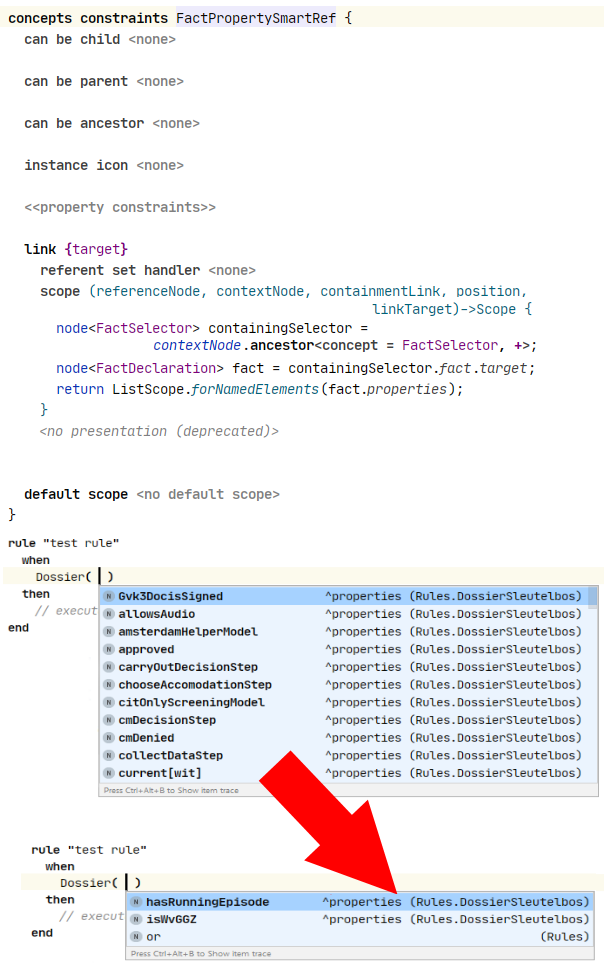
\includegraphics[width=0.66\textwidth]{Sections/images/RSRConstraint_P.png}}
    \caption{RSD scoping constraint}
    \label{fig:RSDConstraint}
\end{figure}

\newpage
\subsection{Drools-Lite Language}
\label{section:DroolsLite}

The RSD served as a useful pilot to demonstrate that different projections could be useful. 
However, it suffered from two significant issues.
Firstly, its limitations as a language were so substantial that it could not handle many necessary scenarios.
Secondly, developers with Drools experience will validate our projections. 
Thus, as RSD would be too alien to them, it would be impractical to use for validation. 
For this reason, we needed to create a projectional language that was much closer to the Drools language.

\begin{figure}[htbp]
    \centering
    \fbox{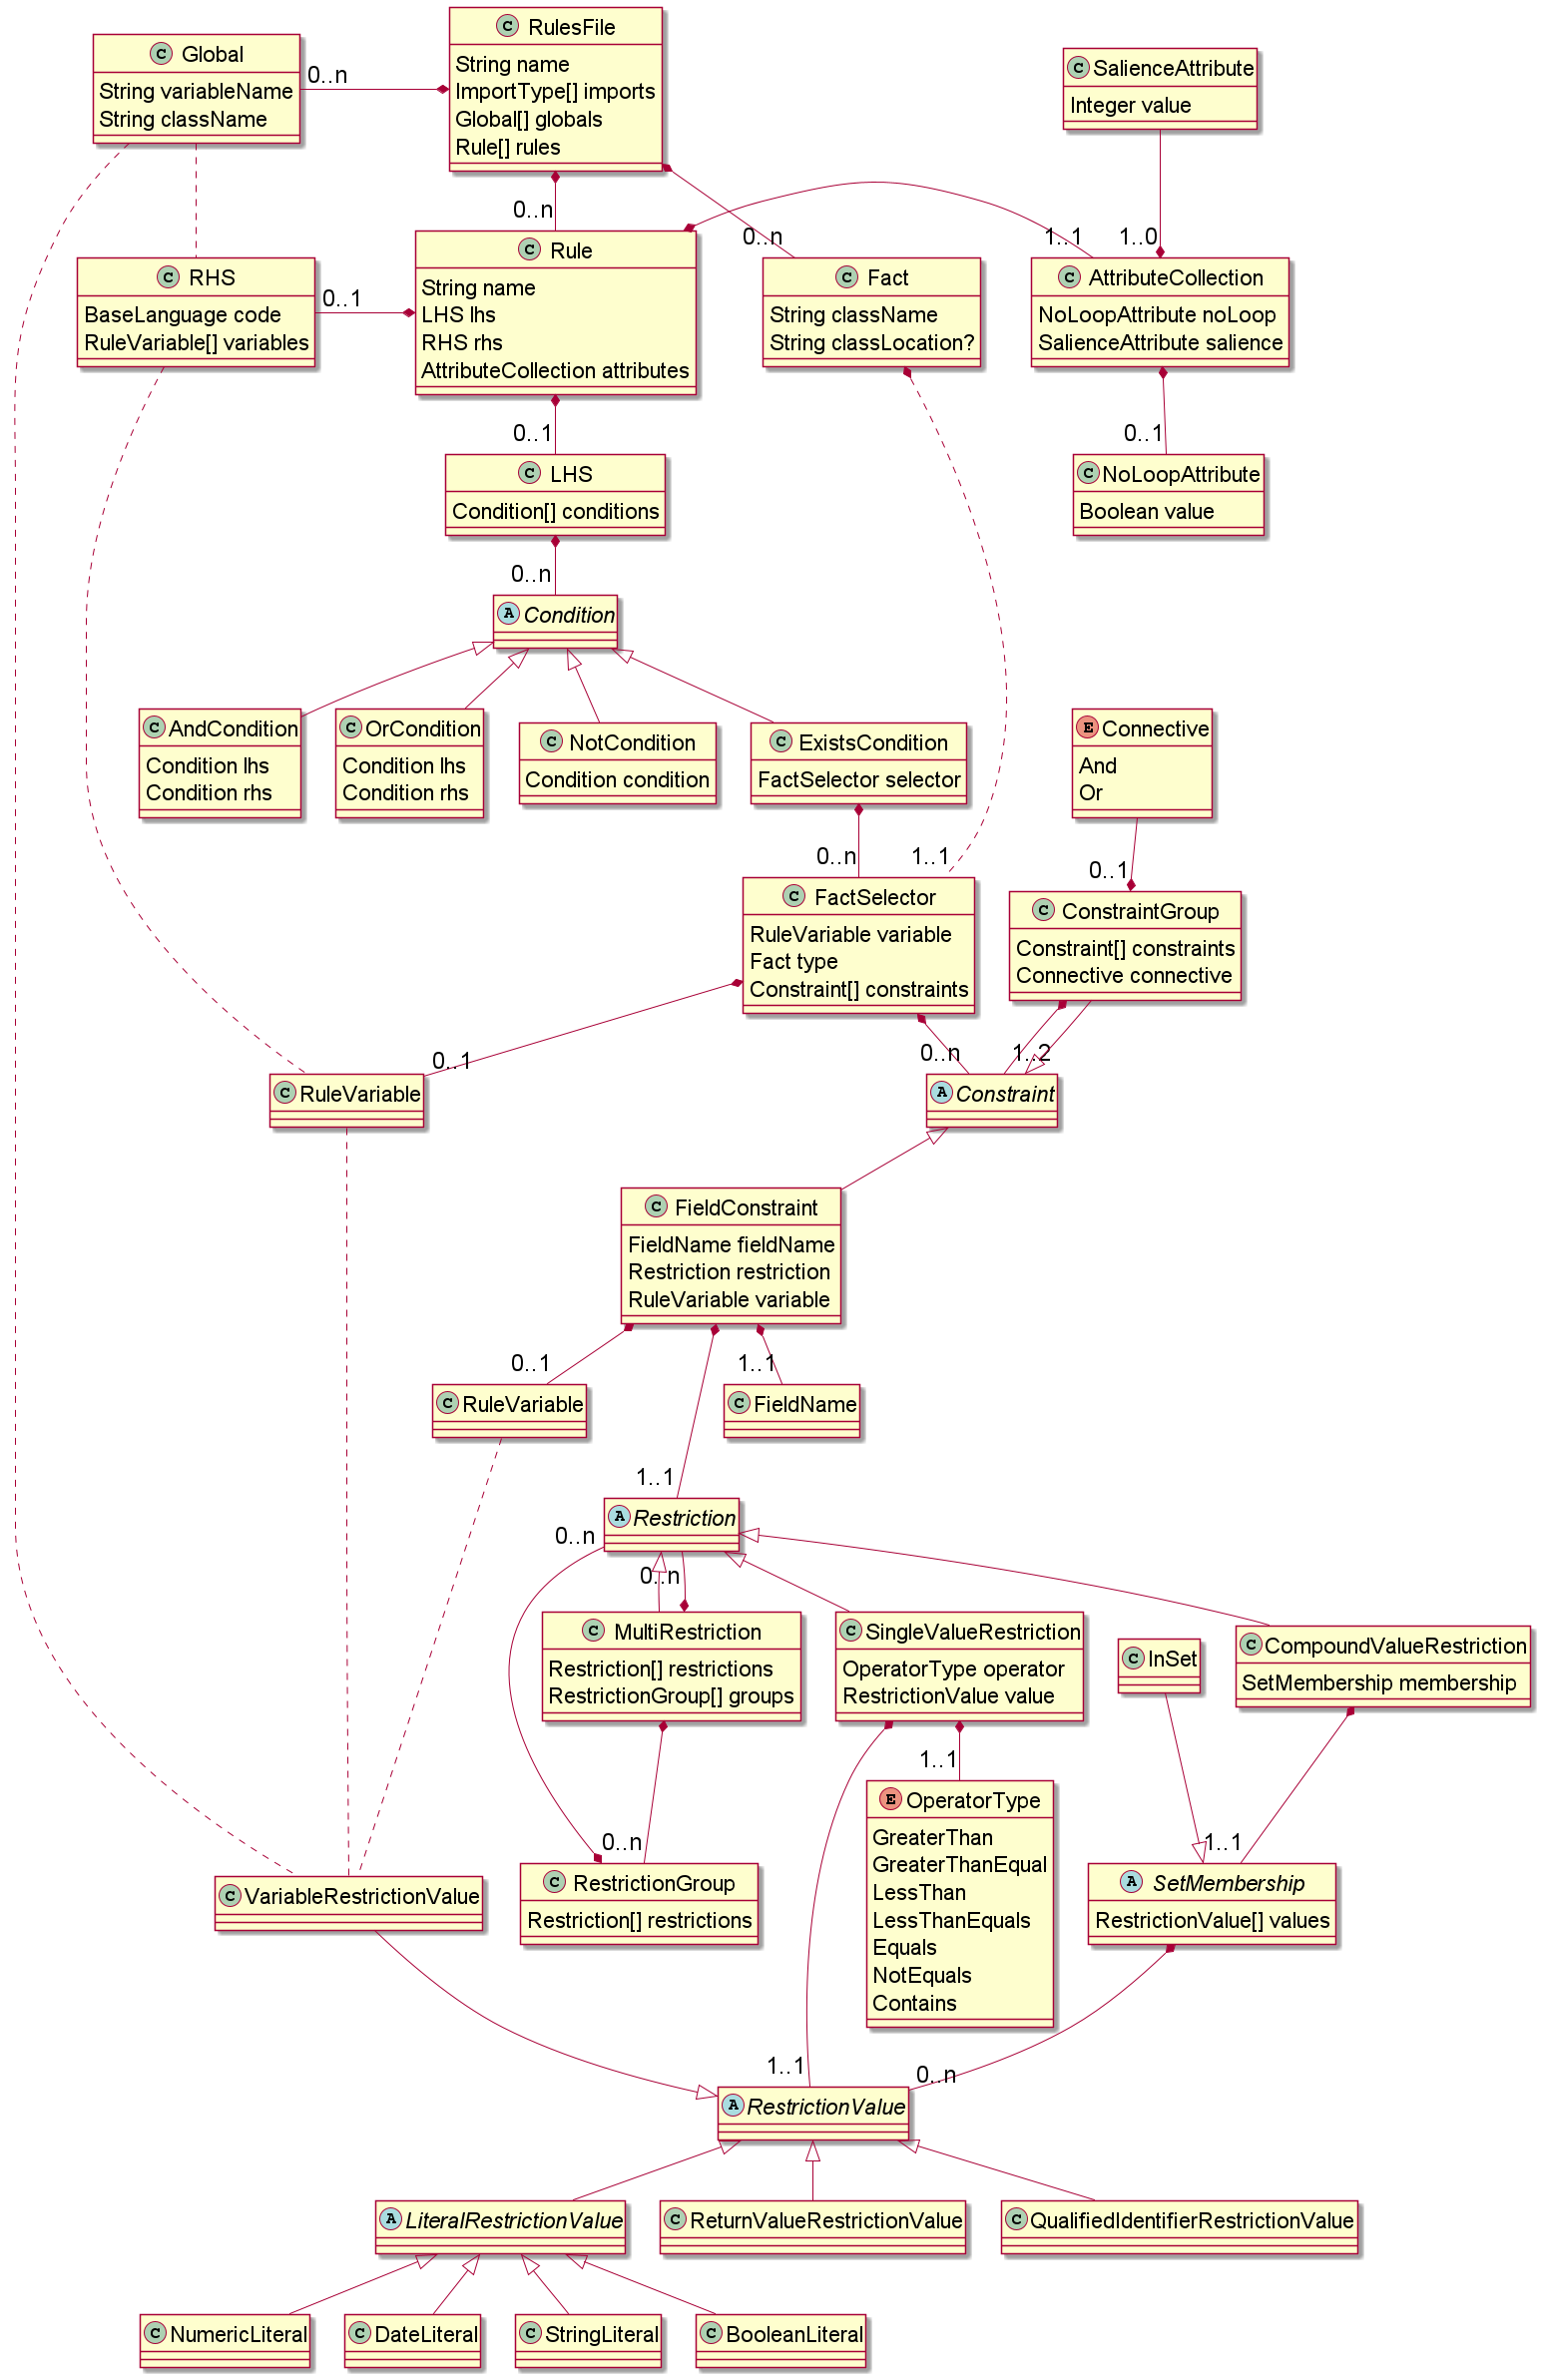
\includegraphics[width=0.90\textwidth]{Sections/images/DroolsLiteStructure.png}}
    \caption{Drools-Lite structure}
    \label{fig:DroolsLiteDiagram}
\end{figure}
 
Our following Language, Drools-Lite, contains many more of the features of Drools.
Our method of selecting the features involved implementing the examples delivered with Drools (including the corrupt politician example shown in section \ref{section:WhatIsDrools}).
We would implement just enough features to complete the examples.
Whenever we had any queries about designing Concepts, we referred to our analysis of the Drools Language, shown in appendix \ref{appendix:DroolsConceptHierarchy}.
We show the preliminary design we achieved using this method in figure \ref{fig:DroolsLiteDiagram} on page \pageref{fig:DroolsLiteDiagram}.
Later, there were some places we diverged a little from our design.
We merged and decoupled our Concepts when we thought it would simplify the code.

\subsubsection{Concepts}

\paragraph{\texttt{RuleFile}} The \texttt{RuleFile} Concept contains \texttt{FactDeclaration} nodes, \texttt{Global} nodes and \texttt{Rule} nodes.
It also contains semantically unimportant empty lines.

\paragraph{FactDeclaration} A \texttt{FactDeclaration} Concept has a ``type'' property.
We implement the ``type'' property using a \texttt{ClassifierType} node from the MPS BaseLanguage.
This implementation allows a \texttt{RuleFile} node to refer to BaseLanguage classes implemented in the same solution or from Java JAR files.

We created a smart reference Concept for this to take advantage of built-in MPS UI functionality.
A smart reference is a node with a single reference of 1:1 cardinality.
The editor builders know how to select which nodes are in scope to display to the developer if one uses this object rather than directly referencing the node it refers to.

\paragraph{FactProperty} In RSD, we had \texttt{FactProperty} nodes as children of \texttt{FactDeclaration} nodes.
Now that our \texttt{FactDeclaration} nodes refer to actual classes (\texttt{ClassifierType}), our \texttt{FactProperty} Concept should reflect this.
To do this, the Concept itself only references an \texttt{InstanceMethodDeclaration}, the MPS BaseLanguage's definition of a method signature.
We scoped the Concept to only show properties associated with a selected \texttt{FactDeclaration}.

Drools interacts with Java objects as if they are Java Beans.
To simulate this, we limited the scope of the properties to just getters, i.e., methods that start with ``get'' or ``is'', and used a Behavior to display them without the ``get'' or ``is'' prefix.
We also made a smart reference for this Concept.

Another option for achieving this is to have wrapped the \texttt{ClassifierType} Concept and referenced its related \texttt{InstanceMethodDeclarations}.
We would have then had to limit the functionality of these items from the BaseLanguage.
Whilst this allows the functionality we wished for, we feel our construction offers decoupling and that, we think, correctly reflects the structure of the language.
Perhaps if we were to redo this, we would have taken the other approach.

\paragraph{\texttt{Global}} Our \texttt{Global} Concepts are very straightforward.
They have a ``name'' property and a BaseLanguage ``type'' child node.
We added a smart reference so that \texttt{Rule} nodes can easily use them.
The reference extended the \texttt{Expression} Concept from the BaseLanguage.
This extension is so that we could use it in the Java code of the Right-hand side.

\paragraph{\texttt{Rule}} Our \texttt{Rule} Concept has three children: an \texttt{AttributeCollection} node, a Right-hand side node and a list of \texttt{AbstractConditions} that make up the Left-hand side.
We created a component to describe the \texttt{Rule} editor for reuse, as we imagined that we would wrap this in other projections.

\paragraph{\texttt{RuleVariables}} The \texttt{FactDeclaration} node referenced by a \texttt{FactSelector} node and the \texttt{FactProperty} referenced by a \texttt{FieldConstraint} node can be bound to \texttt{RuleVariable} nodes.
\texttt{RuleVariable} nodes are scoped to a \texttt{Rule} node.
A \texttt{RuleVariable} Concept has only a \texttt{name} property and a \texttt{Type} child node.
We also create a smart reference for it so that it can be used elsewhere within the \texttt{Rule}.
Like the \texttt{Global} Concept, it extends BaseLanguage's \texttt{Expression} to be available in the Java code of the Right-hand side.

\paragraph{Right-hand side} The right-hand side of the \texttt{Rule}, for the most part, is Java code.
To implement this, we made the right-hand side of the \texttt{Rule} Concept a single \texttt{StatementList} node.
A \texttt{StatementList} Concept is a list of \texttt{Statement} nodes, both from the BaseLanguage.
We chose these because they keep track of, amongst other things, the scope of variables among the statements.

There are some non-Java, Drools specific items that are available to the right-hand side.
Items that had to be useable within the right-hand side were \texttt{Global} references, \texttt{RuleVariable} references and Drools specific functions.
These all extend the \texttt{Expression} Concept from the BaseLanguage.
This extension allows seamless integration with the Java code.

The \texttt{Insert}, \texttt{InsertLogical}, \texttt{Modify}, \texttt{Delete} and \texttt{Halt} Concepts represent the Drools specific required methods.

\begin{figure}[H]
    \centering
    \fbox{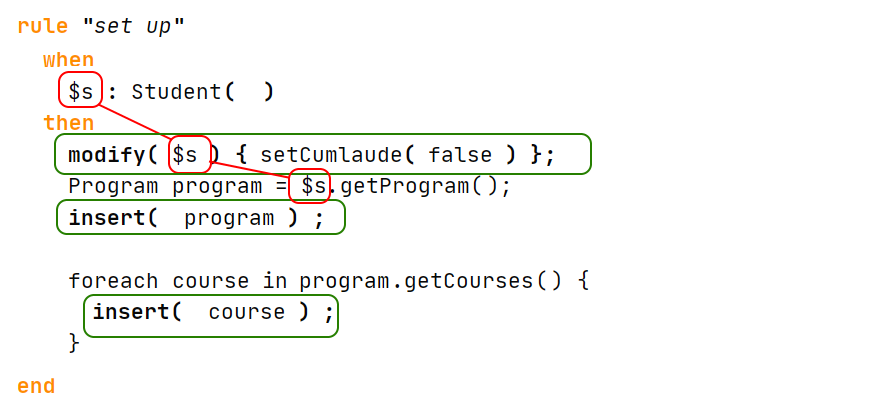
\includegraphics[width=0.70\textwidth]{Sections/images/RHS.png}}
    \caption{RHS}
    \label{fig:RHS}
\end{figure}

Figure \ref{fig:RHS} shows some of the features discussed for the right-hand side, as shown in our default projection.
The right-hand side is the text shown between the ``then'' keyword and the ``end'' keyword.
The figure shows examples of plain Java code, such as assigning to the variable ``program'' and the ``foreach'' loop.
We can also see that Drools-Lite \texttt{RuleVariable} node ``\$s'' is in the Java statements.
We have also highlighted the Drools specific methods placed in the code.
In this case, the \texttt{\textbf{modify}} and \texttt{\textbf{insert}} methods.   

\begin{figure}[H]
    \centering
    \fbox{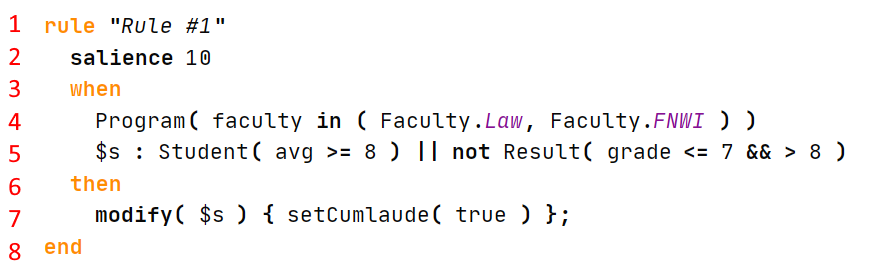
\includegraphics[width=0.85\textwidth]{Sections/images/Rule.png}}
    \caption{Rule}
    \label{fig:Rule}
\end{figure}

\paragraph{\texttt{AttributeCollection}} The \texttt{AttributeCollection} Concept is a container to hold all the attributes that apply to a \texttt{Rule} node.
Initially, we have only implemented the \texttt{NoLoopAttribute} and \texttt{SalienceAttribute} Concepts.
A developer activates these attributes using two intentions we added to the \texttt{Rule} Concept.
On line 2 in figure \ref{fig:Rule}, we can see an example of a \texttt{SalienceAttribute} node added to a \texttt{Rule} on line 2.
\footnote{In figure \ref{fig:Rule}, we added line numbers to this figure to make it easier to talk about.
The keywords ``rule'' on line 1, ``when'' on line 3, ``then'' on line 6, and ``end'' on line 8 have no meaning in the abstract syntax.
We added them to give the developer the same look and feel as a standard Drools file.}

\paragraph{Left-hand side} This is a collection of \texttt{AbstractCondition} nodes.
There are four types of \texttt{AbstractCondition} Concepts.
\texttt{AndCondition}, \texttt{OrCondition}, \texttt{NotCondition} and \texttt{ExistsCondition} Concept.
\texttt{AndCondition}, \texttt{OrCondition}, and \texttt{NotCondition} have one or two children who are also \texttt{AbstractCondition} nodes.
The \texttt{ExistsCondition} Concept contains a \texttt{FactSelector} node.

We added dynamic braces to only show braces around a Condition if it is another Condition's child. 
These braces add visual clarity without adding unnecessary clutter.
We also added some intentions to make it easy to switch between \texttt{ExistsCondition} and \texttt{NotCondition} nodes.

On line 4 in figure \ref{fig:Rule}, the whole line represents an \texttt{ExistsCondition} node.
Line 5 shows an \texttt{OrCondition} node containing an \texttt{ExistsCondition} node and a \texttt{NotCondition} node.
The default editor, through an intention, can make the \texttt{ExistsCondition} visibly explicit with an ``exists'' keyword.
However, the standard practice with Drools developers is to make this implicit, so this is how we show it here.

\paragraph{\texttt{FactSelector}} This always has a reference to a \texttt{FactDeclaration} node.
These are references to the \texttt{FactDeclaration} nodes named ``Program'' in line 4 of figure \ref{fig:Rule} and ``Student'' and ``Result'' from line 5.

Optionally, the \texttt{FactSelector} node can be bound to a variable.
In figure \ref{fig:Rule}, line 5, the \texttt{FactSelector} node referencing the \texttt{FactDeclaration} named ``Student'' is bound to the \texttt{RuleVariable} node named ``\$s''.

The \texttt{FactSelector} Concept also contains a list of constraints on \texttt{FactProperty} references, all of which must return true for a \texttt{FactSelector} node to return true.

\paragraph{Constraints} We have three types of \texttt{AbstractConstraint} Concepts.
\texttt{AndConstraint} and \texttt{OrConstraint} Concepts contain other child constraints.
The \texttt{FieldConstraints} Concept places restrictions on \texttt{FactProperty} references.

\paragraph{FieldConstraints} A \texttt{FieldConstraint} Concept refers to a \texttt{FactProperty} node and can be bound to a variable.
It also has a restriction applied to that \texttt{FactProperty} node.
Using a substitute menu, we wrapped the \texttt{FactPropertySmartRef} Concept.
This substitution automatically creates a \texttt{FieldConstraint} node from the \texttt{FactProperty} node selection by the developer.

There are several types of restrictions and several types of values that they can restrict.

\paragraph{\texttt{RestrictionValues}} The \texttt{AbstractRestrictionValue} Concepts that a \texttt{FactProperty} node can be compared with are as follows:
\begin{itemize}    
    \setlength\itemsep{0em}
    \item \texttt{LiteralRestrictions}: These are \texttt{Integer}, \texttt{Float}, \texttt{String}, \texttt{DateTime} and \texttt{Boolean}.
    \item \texttt{VariableRestrictions}: These can be \texttt{Global} references, \texttt{RuleVariable} references referring to \texttt{FactDeclaration} references from the \texttt{FactSelector} node, or a \texttt{RuleVariable} node from other \texttt{FieldConstraint} nodes.
    \item \texttt{ReturnValue}: This compares to anything expressed as an \texttt{Expression}, which includes referring to constants or values behind qualified identifiers.
\end{itemize}

In figure \ref{fig:Rule}, on line 4, we have the return values ``Faculty.Law'' and ``Faculty.FNWI''.
On line 5, the literal values ``7'' and ``8''.

\paragraph{Restrictions} A \texttt{SingleValueRestriction} Concept compares a \texttt{FactProperty} node against a value.
A \texttt{MultiRestriction} Concept compares a \texttt{FactProperty} node against multiple values, not necessarily using the same comparison for each value.
A \texttt{SetMembership} restriction Concept checks if a \texttt{FactProperty} node is a member or not a member of a group.

In figure \ref{fig:Rule} on line 4 a \texttt{SetMembership} restriction node is shown with the ``in ( Faculty.Law, Faculty.FNWI )'' text.
Line 5 in the first \texttt{FactSelector} node is the \texttt{SingleValue} restriction node represented by ``avg >= 8''.
The second \texttt{FactSelector} node shows a \texttt{MultiRestriction} node using ``grade <= 7 \&\& > 8''.

Thus, we have described the pertinent implementation details of the Drools-Lite language.

\subsection{Wireframes}

There are some potential projections we have conceived for which there is not sufficient time to implement.
We want Drools experts to assess these and thus would like them to appear as realistic as possible to the assessors.

Our solution to this conundrum is to develop these presentations in a wireframing tool.
The wireframe tool we chose was Axure\cite{Axure_ProductPage}.
We chose this because we had previous experience with the product.
Also, it is available to students for free.

We settled on two possible projectional programming aids: Truth table and circuit diagram.
We will discuss these in more detail in the results section.
